\chapter{Peer to Peer Network}
\section{Blockchains and Networking}
A blockchain network is a system that provides ledger and smart contract services to applications without relying on a centralized server or authority. A centralized server can be a single point of failure or a target for censorship, which can compromise the security and availability of the network. Therefore, a blockchain network has the following networking requirements:
\begin{itemize}
    \item 
    The key primitive of the network is to \textbf{broadcast blocks and transactions to all nodes}.\\ Blocks are data structures that contain transactions, which are records of value transfers or contract executions. Transactions are validated and appended to the ledger by consensus algorithms. Broadcasting ensures that all nodes have the same view of the ledger and can verify its integrity.
    \item 
    The network also needs to be \textbf{robust and resilient to node failures or attacks}. \\ Some nodes may go offline due to various reasons, such as power outages, network disruptions, or malicious attacks. The network should be able to tolerate a certain percentage of node failures without affecting its functionality. Moreover, the network should allow new nodes to join and synchronize with the existing nodes, as well as handle node churns and partitions.
\end{itemize}
\subsection{Types of Network Architecture}
There are two types of network architecture:
\begin{enumerate}
    \item \textbf{Client Server} : \\
    This is a type of network architecture where one or more servers store most of the data and resources, and the clients access them through requests. The server is the central authority that controls the network, and the clients are dependent on the server for their functionality.
    \item \textbf{Peer to Peer} :\\
    This is a type of network architecture where each node acts as both a client and a server, and there is no central authority or hierarchy. The nodes share their data and resources directly with each other, without relying on a server.
\end{enumerate}
\begin{figure}[h!]
    \centering
    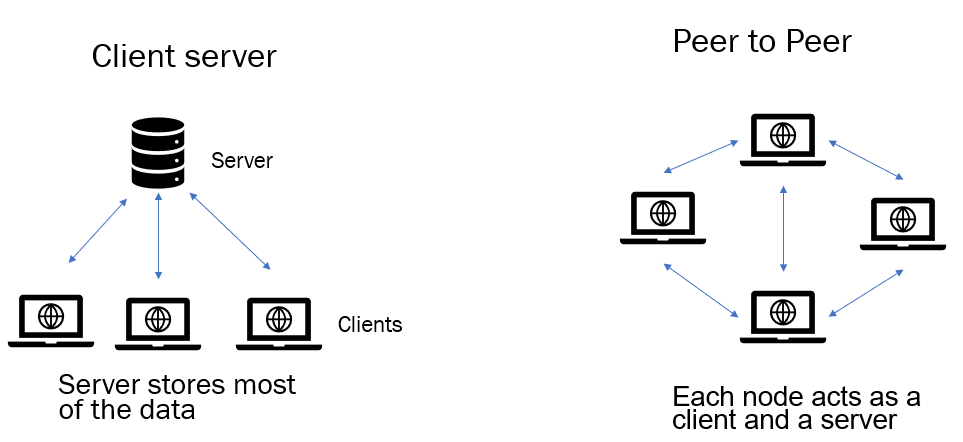
\includegraphics[width=0.6\linewidth]{Fig/04/F1}
    \caption{Types of Network Architecture}
    \label{fig:f1}
\end{figure}
The need for robustness implies that we do not want a client-server relationship; we settle for a peer-to-peer (P2P) network where each node has identical behavior.
\subsection{Overlay Networks}
An overlay network depicts the connections between nodes and is represented as a graph. It abstracts out the physical network switches and routers and defines virtual links between nodes. Two nodes that are connected by a link can exchange messages directly. Those that are not connected by a link must find a path connecting them on this overlay
network in order to communicate messages.
\begin{figure}[h!]
    \centering
    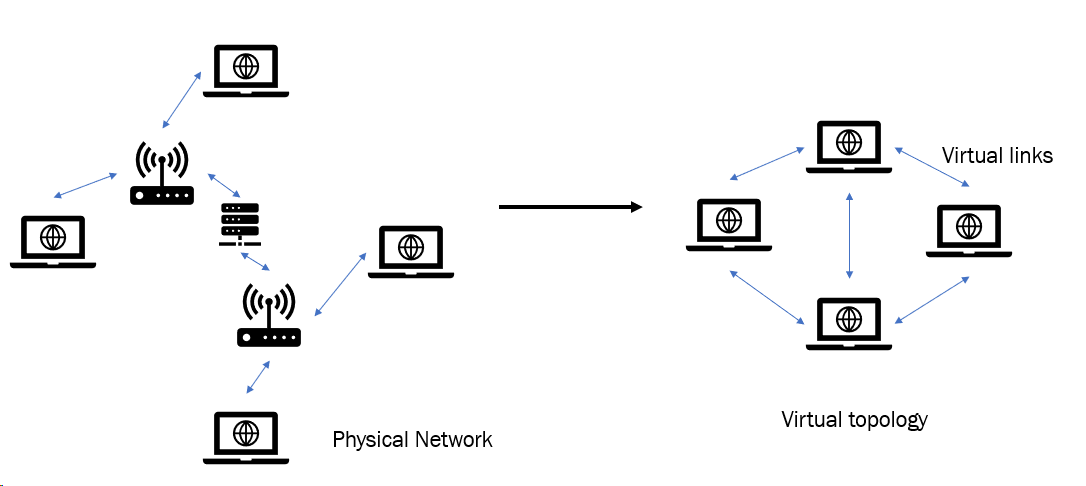
\includegraphics[width=0.7\linewidth]{Fig/04/F2}
    \caption{Overlay Network}
    \label{fig:f2}
\end{figure}\\
There are different ways to classify overlay networks, but one common way is to distinguish between two types of overlay networks
\begin{itemize}
    \item \textbf{structured} : These are overlay networks that have a specific topology or organization, such as a ring, a tree, or a grid. Structured overlay networks, like CHORD, assign an identifier to each node and use that to construct well-defined
    routing rules. These networks are excellent for routing and sending point-to-point messages, a use case not required for Bitcoin. Structured networks are suitable for broadcast, too; any message transmission takes $\mathbb{O}(\log(n))$ hops on CHORD with $\mathbb{O}(\log(n))$ connections per node.
    \item \textbf{unstructured} : These are overlay networks that have no specific topology or organization, and the nodes are connected randomly or based on some criteria, such as proximity, interest, or availability. Unstructured networks like d-regular graphs have no node identifiers; a node connects to d other nodes randomly.
\end{itemize}
Routing point-to-point messages is not feasible because it takes $\mathbb{O}(\log(n))$ hops and requires many peer queries to find the path from point $A$ to point $B$. However, broadcast is very effective using gossip and also takes $\mathbb{O}(\log(n))$ hops. Therefore, the number of hops needed is equal to the structured network with the extra advantage of $\mathbb{O}(1)$ peer connections. That is why the Bitcoin network uses an unstructured d-regular overlay network.
\subsection{Gossip and Flooding}
Gossip and Flooding are two techniques for disseminating information in a network of nodes. Gossip is a technique that randomly sends the information to some of its neighbors, while Flooding sends the information to all of its neighbors. Both techniques can spread the information exponentially and reach all nodes in $\mathbb{O}(\log(n))$ time.\\
Gossip and Flooding can be used to achieve fast and reliable information dissemination in a network, but they differ in terms of efficiency, overhead, and robustness.
\subsection{Expander Graph}
Expander graph is a type of graph that has the property of being well connected but sparse. 
\dfn{Sparse Graph}{A sparse graph $G(V,E)$ is a graph that has a small number of edges compared to the number of vertices, such that $|E| = O(|V|)$, where $|E|$ is the number of edges and $|V|$ is the number of vertices. \\\\
An Expander graph is a sparse graph that is also well connected, such that for any subset $A$ of vertices, the number of vertices outside $A$ that have at least one neighbor in $A$, denoted by $|A|$, is large.}
A gossip message starts with $A(0)$ as the broadcasting node with $|A(0)| = 1$. In the next hop, it will reach $\partial A(0)$ with $|A(1)|$ being at least $(1 + \epsilon)$ times $|A(0)|$. This process repeats and we get $|A(k)|$ being at least $(1 + \epsilon)^k$ times $|A(0)|$ for any $k$. Therefore, the number of steps to get to half the number of nodes is proportional to the logarithm of the number of nodes. It can be proven that the other half of the nodes can also be reached in O(logN) time.

\section{Bitcoin Network}
BBitcoin is a peer-to-peer network that uses TCP protocol to exchange data. In the Bitcoin network:
\begin{itemize}
    \item The codebase limits the number of outgoing connections to eight and the number of incoming connections to 117.
    \item The network has a high churn rate (the rate at which users join or leave the system); therefore, the node must be prepared to connect to new peers.
    \item The node maintains a large list of nodes running Bitcoin in the form of their (IP, port) pair and connects to one of them randomly when a slot becomes available.
    \item The node ensures that the peers it connects to are selected randomly.
\end{itemize}
\subsection{Peer discovery}
A node starts its list of peers by connecting to a group of DNS seed nodes. These are special nodes that provide a list of IP addresses and ports of active nodes in the network. A node can query a DNS seed node to get this list and then try to connect to some of the nodes in the list.\\
The seed nodes are not very distributed; so it is not wise to depend entirely on the peer list given by them. After connecting to the first set of peers, a node requests its peer list using \textbf{getAddr} and \textbf{Addr} messages. The node updates its peer list frequently by swapping peer lists with its peers.
\subsection{Block transmission}
The process of transmitting blocks and transactions involves the following steps:
\begin{enumerate}
    \item A node sends an \textbf{inv} message to its peers, which is an inventory message that tells them what blocks and transactions are available.
    \item When a peer receives an \textbf{inv} message, it checks if it already has the block or the transaction in its local storage. If not, it sends a \textbf{getData} message to the node to get those blocks and transactions.
    \item Optionally, the peer can request only the headers of the blocks first, using a \textbf{getHeaders} message, before asking for the full blocks.
    \item This header-first block transmission can reduce the bandwidth use and prevent invalid blocks from being accepted.
\end{enumerate}
\begin{figure}[h!]
    \centering
    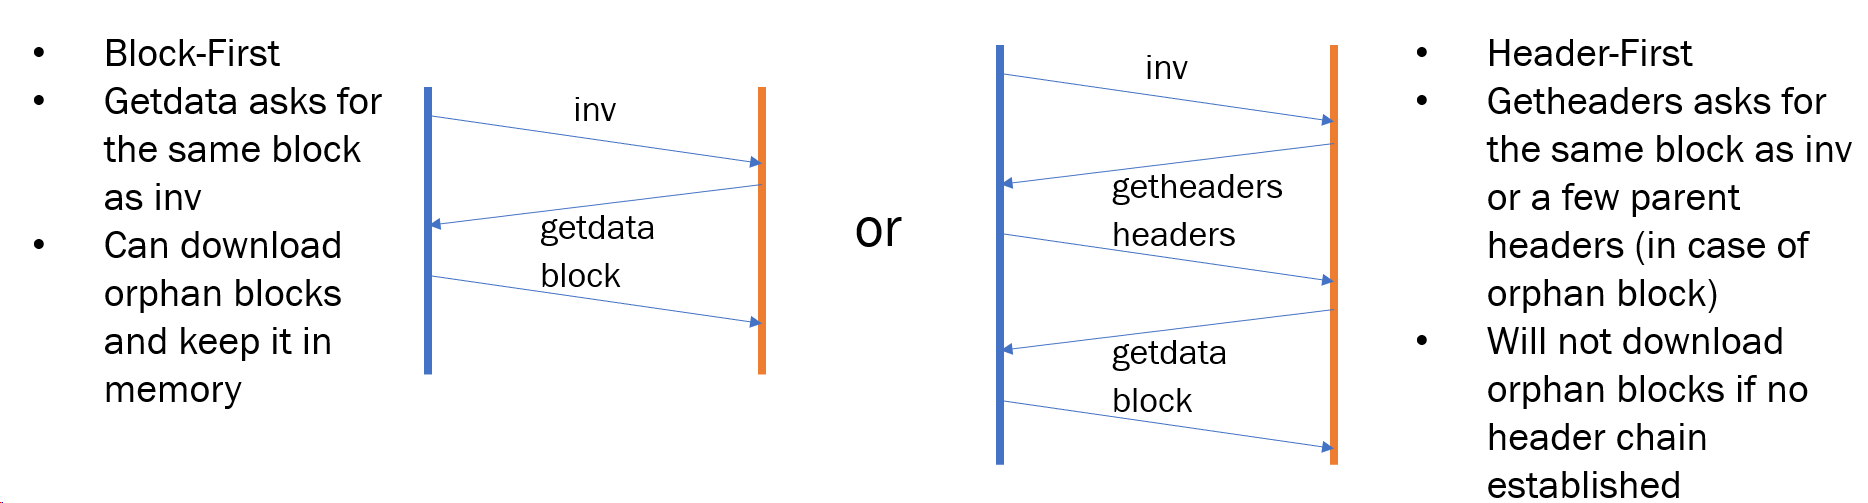
\includegraphics[width=0.8\linewidth]{Fig/04/F3}
    \caption{Block transmission in blockchain network}
    \label{fig:f3}
\end{figure}
\subsection{Data Broadcast}
Now we explain how data, such as transactions, are broadcasted in a peer-to-peer network
\begin{itemize}
    \item Each node maintains a non-persistent memory to store unconfirmed transactions, which are transactions that have not been included in a block yet. This memory is called the mempool.
    \item When a node receives a new transaction, it sends an inv message to its peers, which contains the transaction id ($txid$). The inv message is a way of checking if the peer already has the transaction in its mempool.
    \item If not, the peer sends a get data message to request the full transaction data from the node. The node then sends the transaction data (tx) to the peer.
    \item Some unconfirmed transactions might be removed from the mempool due to various reasons, such as low fees, expiration time, or double-spending.
\end{itemize}
\subsection{Compact Blocks}
Here we discuss two methods of relaying blocks in a peer-to-peer network:
\begin{enumerate}
    \item \textbf{legacy relaying} : \\
    Legacy relaying is the traditional way of sending the full block data to each node.
    \item \textbf{compact block relaying} : \\
    Compact block relaying is a protocol that reduces the amount of bandwidth and latency required to transfer a block that confirms many transactions that the nodes already have in their mempools.
\end{enumerate}
There are some differences between the two methods in terms of the messages exchanged between the nodes. Here are the advantages of compact block relaying over legacy relaying:
\begin{itemize}
    \item Compact block relaying uses shortened transaction identifiers ($txids$) instead of full transaction data, which reduces the size of the block data.
    \item Compact block relaying allows nodes to request only the transactions they are missing from their mempools, which reduces the redundancy of sending transactions twice.
    \item Compact block relaying has two modes: low bandwidth mode and high bandwidth mode.\\ Low bandwidth mode minimizes bandwidth usage by asking for permission before sending a compact block.\\ High bandwidth mode reduces the latency by sending a compact block as soon as possible without asking for permission.
    \item Compact block relaying can verify the proof of work (PoW) from the block header before requesting the full block data, which prevents invalid blocks from being accepted.
\end{itemize}
\begin{figure}[h!]
	\centering
	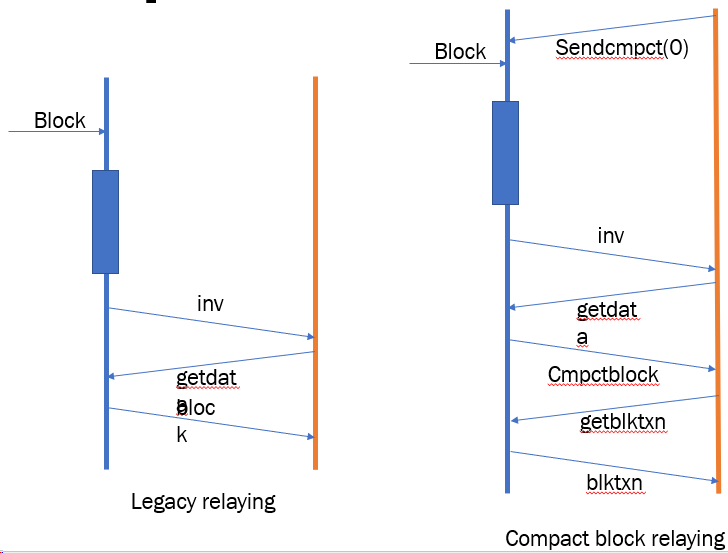
\includegraphics[width=0.6\linewidth]{Fig/04/F4}
	\caption{Compact Block}
	\label{fig:f4}
\end{figure}
There is a trade-off between capacity and propagation delay in a peer-to-peer network. \textbf{Capacity} (C) is the maximum amount of data that can be transmitted in a given time, measured in bits per second (bps). \textbf{Propagation delay} (D) is the time it takes for a signal to travel from one node to another, measured in seconds. The end-to-end delay, which is the total time it takes for a block to reach all nodes in the network, increases with the increase in block size. This is because larger blocks take longer to transmit and verify, which can cause congestion and orphaning. Therefore, there is a trade-off between increasing the capacity and reducing the propagation delay of the network. This increase in delay affects the system in the following ways:
\begin{itemize}
    \item Wasted Hash power
    \item Forking
\end{itemize}
\subsection{Disadvantages of current p2p network}
\begin{itemize}
    \item \textbf{Efficiency:} \\ It requires a lot of communication between nodes. The total communication is proportional to the number of nodes (N) and the average degree of connectivity (d). This means that as the network grows, the communication overhead also increases, which can affect the performance and scalability of the system.
    \item \textbf{Privacy:} \\ It can link the transaction source to the IP address of the node that broadcasts it. This means that anyone who monitors the network traffic can potentially identify the sender and receiver of a transaction, which can compromise their anonymity and privacy.
    \item \textbf{Security:} \\ It allows for plausible deniability for forking. Forking can cause inconsistency and double-spending. Plausible deniability means that a node can claim that it did not receive a valid block from another node, even if it did, and create a fork on purpose. This can be used as an attack strategy to disrupt the consensus and integrity of the system.
\end{itemize}

\section{Geometric Random Network}
The current network topology is based on random IP addresses, which are not related to geographic distances. This means that nodes may be connected to peers that are far away from them, which can increase the latency and bandwidth usage of the network. \\\\
A better network topology would be based on a \textbf{geometric random network}, which is a network where nodes are placed according to some geometric criteria, such as proximity or similarity. This way, nodes can connect to peers that are closer or more relevant to them, which can improve the efficiency and performance of the network. The challenges are creating a self-adapting network topology based on measurements, such as latency, bandwidth, or trust. This means that nodes can dynamically adjust their connections based on the changing conditions and preferences of the network.

\subsection{Perigee}
Perigee is a self-adaptive network topology algorithm for peer-to-peer networks. Perigee is a decentralized algorithm that selects neighbors based on past interactions. It aims to retain neighbors that relay blocks fast and disconnect from neighbors that do not relay blocks fast. It also explores unseen neighbors to discover new potential connections.\\\\
`Perigee is motivated by the multi-armed bandit problem, which is a problem of finding the optimal strategy for choosing among several options with uncertain rewards. Perigee tries to balance exploration and exploitation, which means finding new neighbors and using existing neighbors, respectively. Perigee can improve the efficiency and performance of the peer-to-peer network by reducing latency and bandwidth usage.

\subsubsection{Algorithm}
The Perigee Algorithm works as follows:
\begin{itemize}
    \item It assigns scores for each subset of neighbors based on how fast they relay blocks.
    \item It retains the subset of neighbors with the best score and disconnects the node that is not in the subset.
    \item It forms a connection to a random neighbor to explore new potential connections.
\end{itemize}
\begin{figure}[h!]
	\centering
	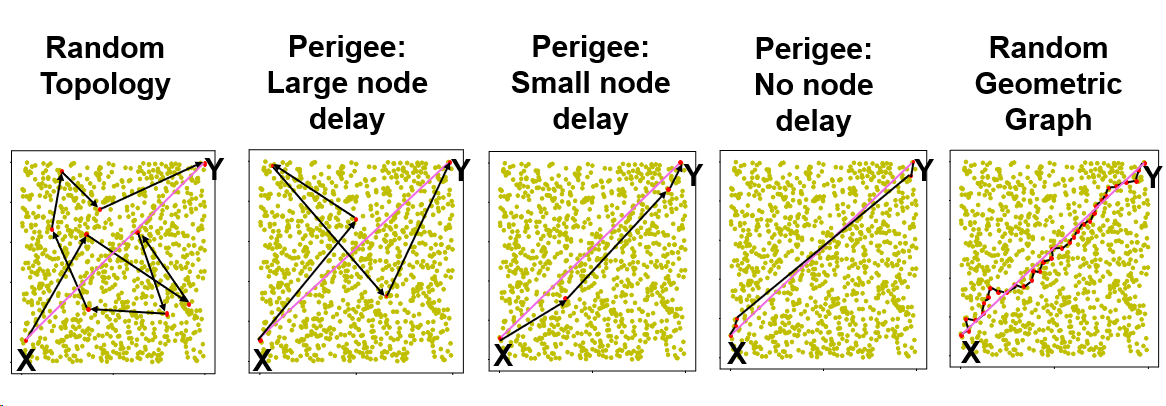
\includegraphics[width=\linewidth]{Fig/04/F5}
	\caption{Performance of Perigee}
	\label{fig:f5}
\end{figure}
\section{Efficient Networking}
Efficient networking is the ability to transmit and receive data in a fast, reliable, and scalable way. There are three aspects of efficient networking:
\begin{enumerate}
   \item \textbf{Trusted networks} : \\
   Trusted networks are networks where nodes can trust each other to relay valid and timely data. Trusted networks can improve the efficiency of the network by reducing the overhead and redundancy of data transmission. However, trusted networks also pose some risks, such as centralization and censorship.
   \item \textbf{Privacy} : \\
   Privacy is the ability to protect the identity and activity of nodes from external observers. Privacy can improve the efficiency of the network by reducing the exposure and vulnerability of nodes. However, privacy also poses some challenges, such as linking transaction source to IP addresses and plausible deniability for forking.
   \item \textbf{Security} : \\
   Security is the ability to prevent and resist attacks from malicious nodes or adversaries. Security can improve the efficiency of the network by maintaining the integrity and consistency of the data. However, security also poses some difficulties, such as eclipse attacks and plausible deniability for forking.
\end{enumerate}
\subsection{FRN (Fast relay network)}
FRN (Fast relay network) is an example of a trusted network model, which is a hub and spoke model where miners connect to FRN servers. FRN servers are trusted servers that are fast and efficient in relaying blocks and transactions. FRN servers can reduce the latency and bandwidth usage of the network by filtering and compressing the data. However, FRN servers also pose some risks, such as centralization, censorship, and single point of failure.
\begin{figure}[h!]
   \centering
   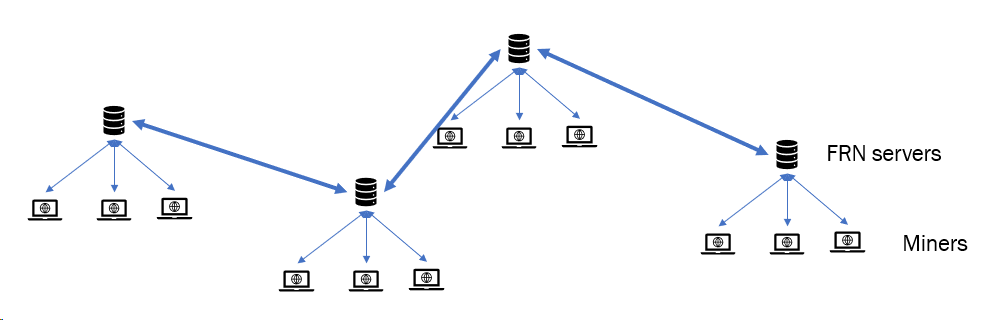
\includegraphics[width=0.7\linewidth]{Fig/04/F6}
   \caption{FRN}
   \label{fig:f6}
\end{figure}
\subsection{Trusted Networks: Falcon}
Falcon network routing is based on the idea of cut-through routing, which is a method of forwarding data packets as soon as their headers are verified, without waiting for the whole packet to arrive. This can reduce the latency and bandwidth usage of the network, as well as the risk of forking and double-spending. Falcon network routing uses a set of trusted servers, called FRN servers, to relay data packets between nodes.\\\\
\textbf{Cut through routing} is the way of sending data packets from point a to point b, where each node verifies the header of the packet and forwards it to the next node without waiting for the whole packet to arrive. The diagram shows that cut-through routing has lower latency than legacy routing, which is represented by the distance between the green lines and the red lines in the diagram. The diagram also shows that cut-through routing uses FRN servers to relay data packets between nodes.
\begin{figure}[h!]
   \centering
   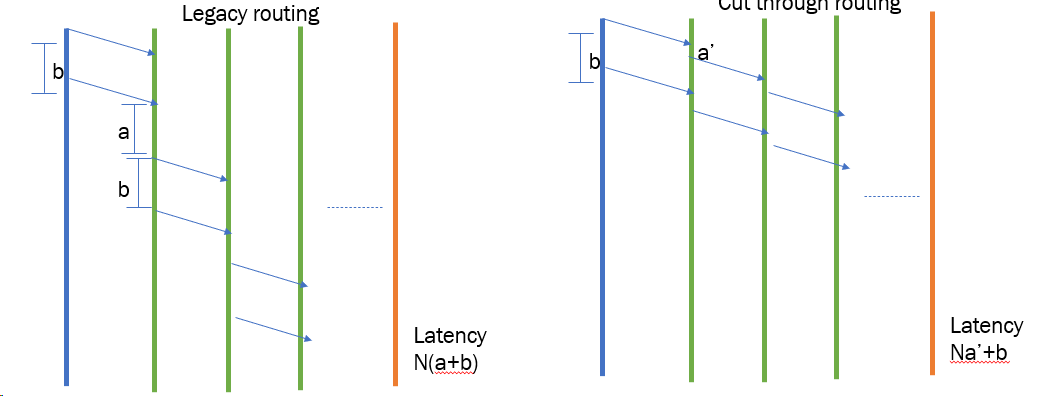
\includegraphics[width=0.7\linewidth]{Fig/04/F7}
   \caption{Legacy routing vs. Cut through routing}
   \label{fig:f7}
\end{figure}
\section{Network Anonymity and Privacy}
Blockchains are systems where the data structure of the blockchain is shared and visible to all participants. For example, in a cryptocurrency, the blockchain records every transaction that ever happened in the currency. However, this also means that the blockchain can contain sensitive data of users, such as their identities and balances. This can raise privacy concerns for users who do not want their data to be public. Therefore, privacy is an important issue in blockchains. How can users achieve privacy in blockchains?\\\\
Bitcoin and most other cryptocurrencies use pseudonymous identifiers to protect the privacy of users. Each user has one or more pseudonyms, which is a public key that they use to participate in the system. The blockchain only shows the transaction patterns of each pseudonym, not the real identity of the user. However, this system is not very secure, because there are ways to link the pseudonyms to the user’s real identity, especially if there is extra information available. These are called de-anonymization attacks, and they can expose the user’s sensitive data.

\subsection{Network De-anonymization Problem}
The network de-anonymization problem is the challenge of finding the real identities of users who participate in a network that uses anonymization techniques. Anonymization techniques are methods that hide the personal information of users, such as their names and locations, by using random or fake identifiers. Anonymization techniques are supposed to protect the privacy of users, but they can be broken by attackers who have access to some extra information or techniques. The network de-anonymization problem can be modeled using a graph, where nodes represent users and edges represent connections between them. The attacker’s goal is to guess which node in the anonymized graph corresponds to which user in the original graph. The attacker can use different methods, such as eavesdropper adversaries or botnet adversaries, to collect and analyze data from the network. Eavesdropper adversaries are attackers who listen to all or most of the network traffic and use metadata and topology information to infer the source of a message. Botnet adversaries are attackers who control a set of compromised nodes that participate in the network normally and share information. The network de-anonymization problem is a difficult and important problem for network security and privacy.\\\\
There are two main types of attackers in network de-anonymization:
\begin{enumerate}
	\item \textbf{Eavesdropper attackers} :\\ Eavesdropper attackers are attackers who connect to all or most of the nodes in the network and listen to their communications. They look like normal nodes to the honest nodes, who relay messages to them as usual. Eavesdropper attackers can collect metadata, such as timestamps and IP addresses, from the messages they receive. They can also use information about the network topology, such as the connections between nodes, to guess the source of a message. Eavesdropper attackers usually do not send any messages; they only observe and analyze the messages they receive.
	\item \textbf{Botnet attackers} : \\
	Botnet attackers are attackers who control a set of compromised nodes that act like normal nodes in the network. They can accept and relay messages from other nodes, but they also share information with each other. Botnet attackers can have limited visibility into the network, depending on how many nodes they control and how they are connected. Botnet attackers can also inject fake or modified messages into the network to confuse or mislead other nodes.
\end{enumerate}
\begin{figure}[h!]
	\centering
	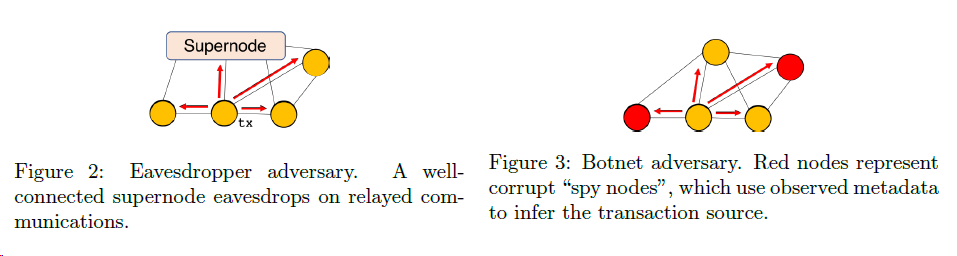
\includegraphics[width=0.7\linewidth]{Fig/04/F8}
	\caption{Eavesdropper adversary (Left graph) - Botnet adversary (Right graph)}
	\label{fig:f8}
\end{figure}
De-anonymization algorithms are methods that can break the privacy of users who participate in a network that uses anonymization techniques. Anonymization techniques are ways of hiding the personal information of users, such as their names and locations, by using random or fake identifiers. However, these techniques can be defeated by attackers who have access to some extra information or techniques. De-anonymization algorithms are based on the idea of centrality or symmetry, which means that the source of a message is usually located at the center of a disc-shaped region on the network graph. The attackers can use metadata and topology information to infer the shape of the disc and identify the central node with a high probability. These algorithms show that diffusion, which is a common way of spreading messages on the network, is not very good at protecting the anonymity of users at the network level. Therefore, there is a need for alternative spreading protocols that can protect the anonymity of users.

\subsection{Flooding Protocol}
 Flooding protocols are methods of sending packets to all nodes in a network by having each node rebroadcast the packets it receives. Flooding protocols can be useful for applications such as firmware updates, routing information, and multicast forwarding. However, flooding protocols can also cause problems such as network congestion, packet loss, and high energy consumption.\\\\
 There are two flooding protocols:
 \begin{enumerate}
    \item \textbf{Trickle} : \\
    Trickle uses a \textbf{polite gossip} policy to control the send rates of nodes. Trickle divides time into intervals and each node maintains a counter of how many consistent packets it has heard from its neighbors. If the counter is below a threshold, the node transmits its packet with a high probability. Otherwise, the node transmits its packet with a low probability. This way, Trickle ensures that nodes hear enough packets to stay consistent, but not too many to cause redundancy.
    \item \textbf{Diffusion} : \\
    Diffusion uses an exponential backoff mechanism to reduce the send rates of nodes. Diffusion assigns each node an exponent value based on its hop distance from the source node. The exponent value determines how long the node waits before transmitting its packet. The closer the node is to the source, the smaller the exponent value and the shorter the waiting time. The farther the node is from the source, the larger the exponent value and the longer the waiting time. This way, Diffusion reduces the number of collisions and retransmissions in the network and improves the reliability and efficiency of packet delivery.
 \end{enumerate}
\begin{figure}[h!]
    \centering
    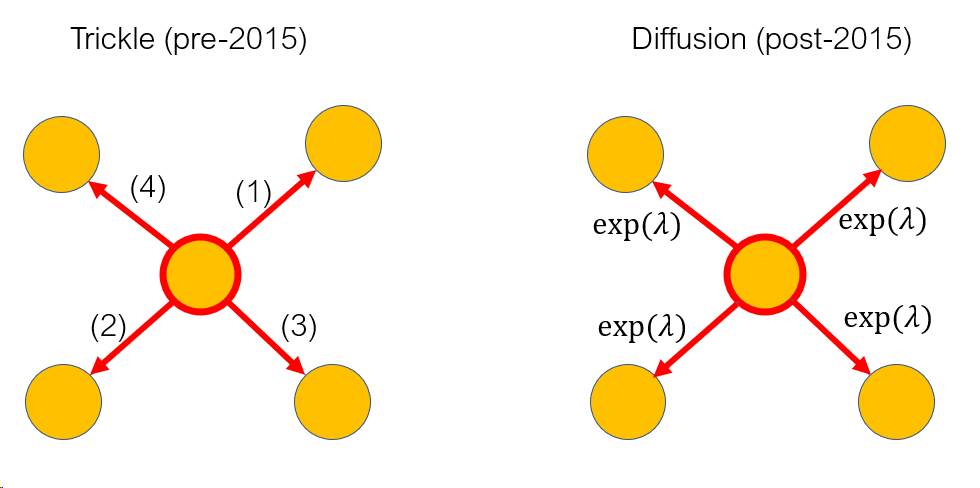
\includegraphics[width=0.6\linewidth]{Fig/04/F10}
    \caption{Flooding Protocols}
    \label{fig:f10}
\end{figure}
Figure \ref{fig:f11} shows that Trickle has a higher probability of detection than Diffusion for any given number of eavesdropper connections. This means that Trickle is more effective in identifying and reporting eavesdropper connections than Diffusion.
\begin{figure}[h!]
    \centering
    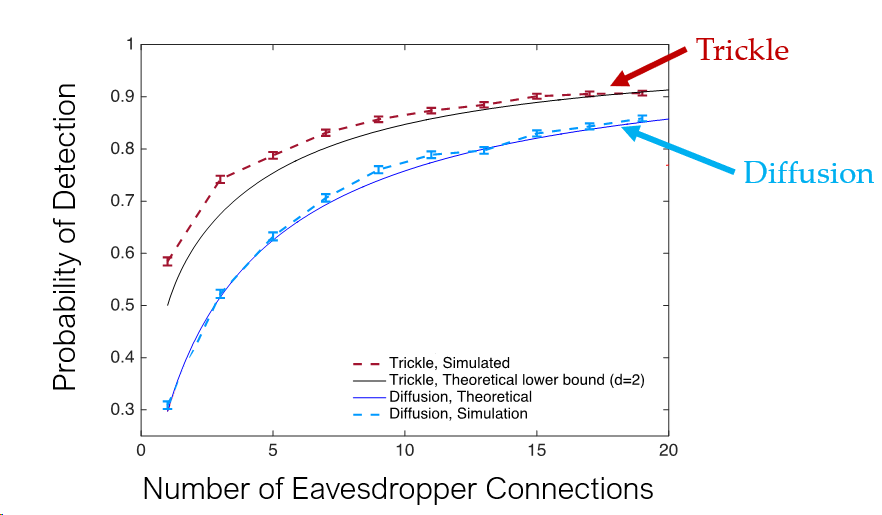
\includegraphics[width=0.7\linewidth]{Fig/04/F11}
    \caption{Performance of Trickle and Diffusion}
    \label{fig:f11}
\end{figure}\\
Diffusion does not have (significantly) better anonymity properties than a trickle.
 
 \subsection{Anonymity in Botnet adversarial model}
 Anonymity is the degree to which a user’s identity and transactions are hidden from other users and observers. Anonymity can be measured by two factors: recall and precision. Recall is the probability that a user’s transactions are detected by an observer, while precision is the accuracy of the observer’s detection.
 \begin{figure}[h!]
    \centering
    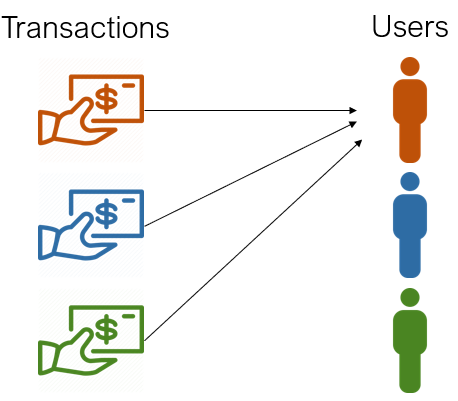
\includegraphics[width=0.25\linewidth]{Fig/04/F12}
    \caption{Mapping $M$}
    \label{fig:f12}
 \end{figure}
 Recall can be calculated using the following formula
 \begin{align*}
    \frac{1}{n}\sum_v 1\{M(v' \, s \, \text{tx}) = v\}
 \end{align*}
 where $n$ is the number of honest users in the network, $v$ is a user index, $M(v' \, s \, \text{tx})$ is the mapping function that assigns a user’s transactions to a user index, and $1\{M(v' \, s \, \text{tx}) = v\}$ is an indicator function that returns 1 if the mapping is correct and 0 otherwise.\\\\
 The formula for calculating precision is :
 \begin{align*}
    \frac{1}{n}\sum_v \frac{1\{M(v' \, s \, \text{tx}) = v\}}{\text{\# tx mapped to } v}
 \end{align*}
Our goal is to design a distributed flooding protocol that minimizes the maximum precision and recall achievable by a computationally unbounded adversary. \\
\begin{figure}[h!]
    \centering
    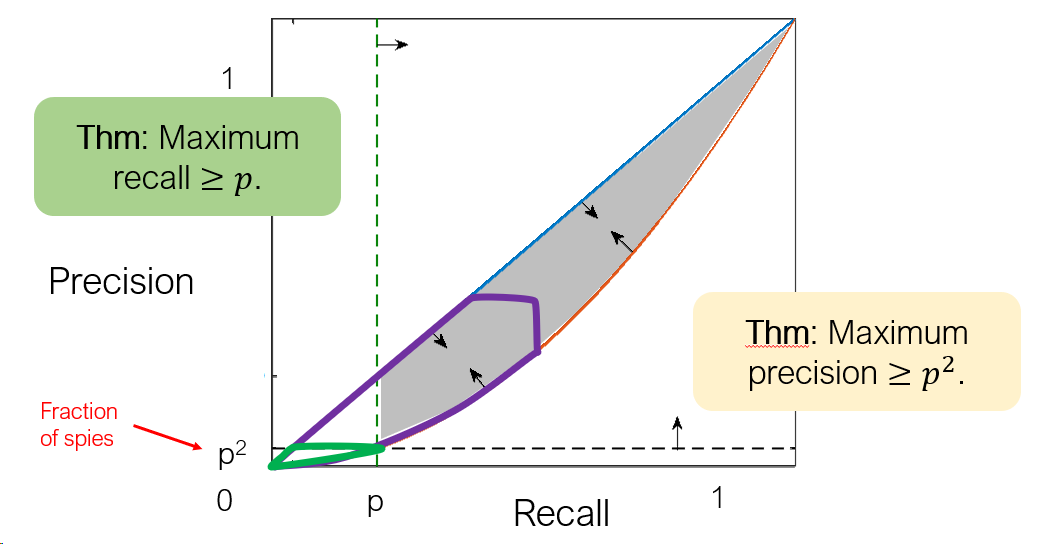
\includegraphics[width=0.5\linewidth]{Fig/04/F13}
    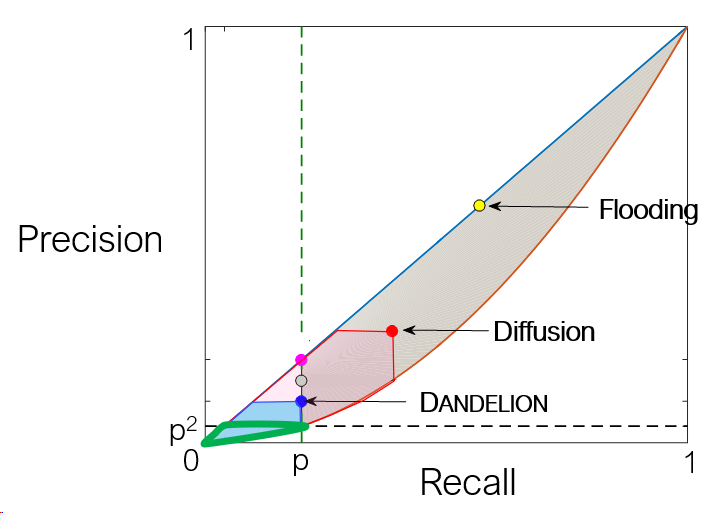
\includegraphics[width=0.4\linewidth]{Fig/04/F14}
    \caption{Fundamental Limits}
    \label{fig:f13}
\end{figure}\\
Figure \ref{fig:f13} implies that we can’t have high precision-low recall and vice versa.

\subsection{Dandelion}
One of the main insights from studying how information spreads is that we need to make the communication protocol asymmetric, so that the adversary cannot easily figure out the message. This is the idea behind the Dandelion P2P network protocol, which has two stages:
\begin{enumerate}
    \item a \textbf{stem stage (or anonymity stage)} : \\
    In the stem stage, each node sends each message in a random direction. This stage lasts for a random number of hops
    \item a \textbf{fluff stage (or diffusion stage)} : \\
    In the fluff stage, the message is diffused to the whole network by broadcasting it
\end{enumerate} 
The stem stage provides anonymity, while the fluff stage ensures fast and reliable delivery.
\begin{figure}[h!]
    \centering
    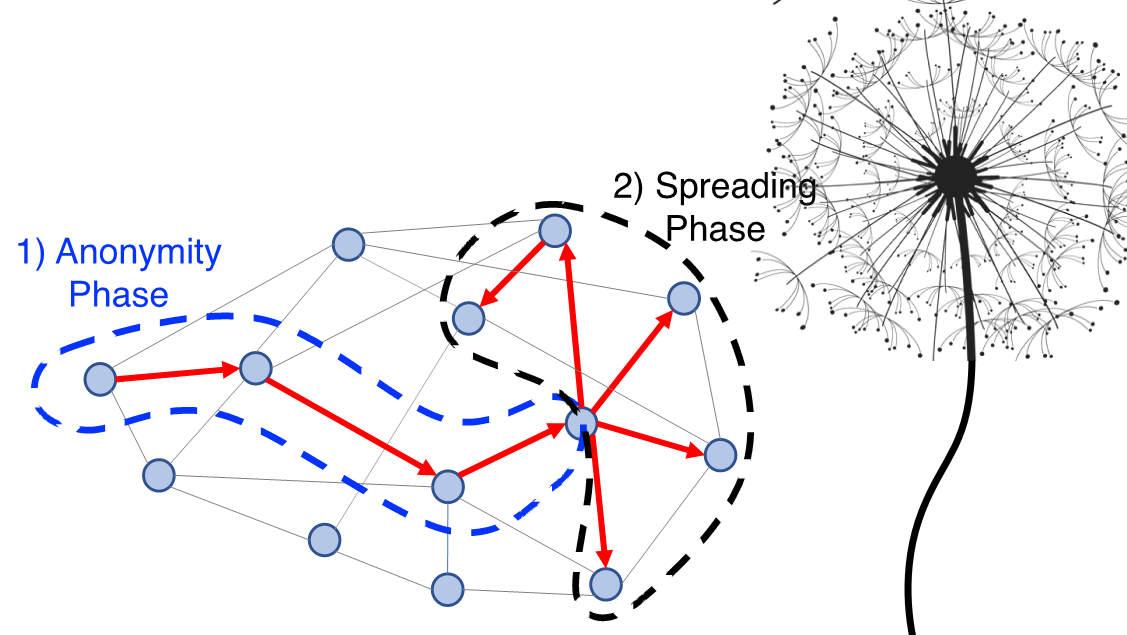
\includegraphics[width=0.6\linewidth]{Fig/04/F9}
    \caption{Spreading Protocol: Dandelion}
    \label{fig:f9}
\end{figure}
We will describe the Dandelion protocol in more detail next. Dandelion works in epochs that are not synchronized; each node changes its epoch when its internal clock reaches a random value (in practice, this will be a few minutes). Within an epoch, the main algorithmic components of Dandelion are:
\begin{enumerate}
    \item \textbf{Anonymity graph:}\\ The random walk happens on a layer of the P2P graph called the anonymity graph. This layer should be either a random cycle graph (i.e., a graph with two edges per node) or a graph with four edges per node. This graph with four edges per node is created from the P2P graph by having each node pick (up to) two of its outgoing edges, without repeating, randomly as Dandelion relays. This does not make an exact graph with four edges per node, but a close one. Each time a node moves to the next epoch, it chooses new Dandelion relays.
    \item \textbf{Sending of a node’s transactions:}\\ Each time a node creates a transaction, it sends the transaction in the stem phase along the same random edge on the anonymity graph. If the anonymity graph is a cycle, there is only one edge per node; otherwise, the node must pick one of its two edges.
    \item \textbf{Relaying of other nodes’ transactions}: \\  Each time a node gets a transaction in the stem phase from another node, it either passes the transaction on or broadcasts it. The decision to broadcast transactions is pseudo-random and is based on a hash of the node’s own identity and epoch number. Note that the choice to broadcast does not depend on the transaction itself—in each epoch, a node is either a broadcaster or a passer for all passed transactions. If the node is not a broadcaster in this epoch (i.e., it is a passer), then it passes transactions pseudo-randomly; each node assigns each of its incoming edges in the anonymity graph to an outgoing edge in the anonymity graph (with repetition). This assignment is chosen at the start of each epoch and determines how transactions are passed.
    \item \textbf{Robustness mechanism}:\\ Each node keeps track, of each transaction in the stem phase that it sends or passes on, whether the transaction comes back as a transaction in the fluff phase within some random time. If not, the node begins to broadcast the transaction.
\end{enumerate}
Dandelion spreading can achieve the lowest possible recall for any given fraction of spies in the network. 
\thm{Recall of Dandelion}{Dandelion spreading has an optimally low maximum recall of \begin{align*}
        p + O \left(\frac{1}{n}\right)
    \end{align*}.}
The theorem implies that no algorithm can reduce the accuracy of detection by an adversary below this bound.
\thm{Precision of Dandelion}{Dandelion has a nearly-optimal 
    maximum precision of \begin{align*}
        \frac{2p^2}{1-p} \, \log\left(\frac{2}{p}\right) + O \left(\frac{1}{n}\right) \quad \text{ for } p < \frac{1}{3}
    \end{align*}
}
Figure \ref{fig:f15} is a timeline chart that shows the evolution of privacy technologies in cryptocurrencies.
\begin{figure}[h!]
    \centering
    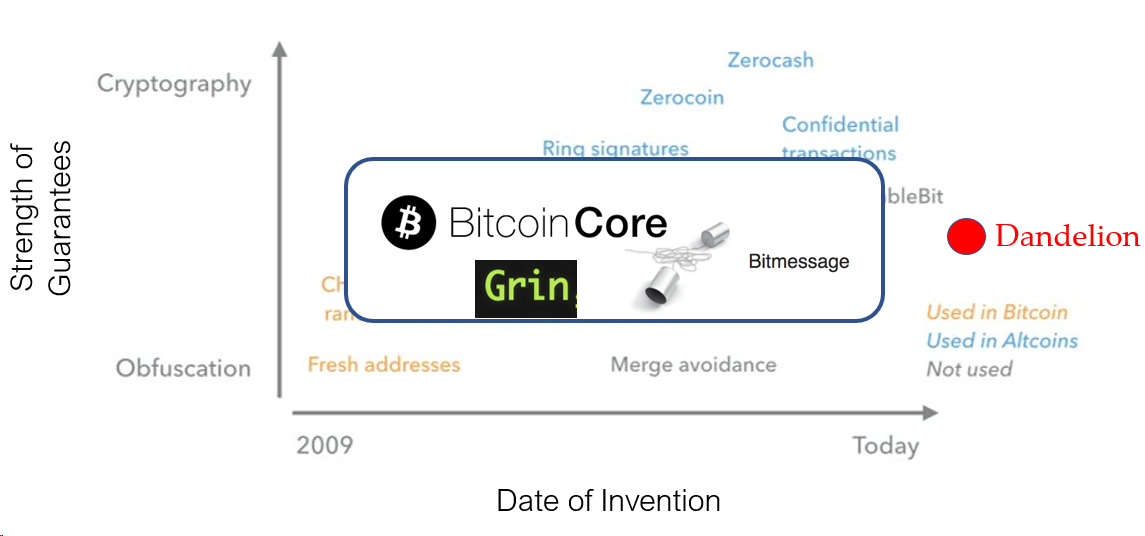
\includegraphics[width=0.75\linewidth]{Fig/04/F15}
    \caption{Evolution timeline}
    \label{fig:f15}
\end{figure}